\documentclass[aspectratio=169]{beamer}
\usepackage[english]{babel}				% Set language
\usepackage[utf8]{inputenc}			% Set encoding
\usepackage{tikz}
\usepackage{svg}

\usepackage{ifthen}

\usetikzlibrary{calc}

\mode<presentation>						% Set options
{
  \usetheme{default}					% Set theme
  \usecolortheme{default} 				% Set colors
  \usefonttheme{default}  				% Set font theme
  \setbeamertemplate{caption}[numbered]	% Set caption to be numbered
}


% emojis
\usepackage{fontawesome}
%\usepackage{fontspec}
%\newfontfamily\DejaSans{DejaVu Sans}

%\usecolortheme[named=UBCblue]{structure}
\setbeamercolor{math text}{fg=black!30!blue}

% Uncomment this to have the outline at the beginning of each section highlighted.
%\AtBeginSection[]
%{
%  \begin{frame}{Outline}
%    \tableofcontents[currentsection]
%  \end{frame}
%}

\usepackage{graphicx}					% For including figures
\usepackage{booktabs}					% For table rules
\usepackage{hyperref}					% For cross-referencing
\usepackage[backend=biber]{biblatex}
\usepackage{csquotes}
\usepackage{bookmark}
\usepackage{colortbl}                   % For color line
\usepackage{framed}                     % For frames

\beamertemplatenavigationsymbolsempty
\setbeamertemplate{footline}[frame number]

\setbeamerfont{author}{size=\large}
\setbeamerfont{date}{size=\scriptsize}
\setbeamercolor{date}{fg=gray}
\defbeamertemplate*{title page}{customized}[1][]
{
  \centering
  \vspace{1cm}
  \usebeamerfont{title}\textbf{\inserttitle}\par
  \bigskip
  \usebeamerfont{author}\insertauthor\par
  \medskip
  \usebeamercolor[fg]{date}\usebeamerfont{date}\insertdate\par
}


\definecolor{myred}{RGB}{176, 38, 0}
\definecolor{myorange}{RGB}{255, 170, 0}
\definecolor{myblue}{RGB}{0, 157, 196}
\definecolor{mygreen}{RGB}{0, 140, 65}
\newcommand{\bred}[1]{\textcolor{myred}{\textbf{#1}}}
\newcommand{\borange}[1]{\textcolor{myorange}{\textbf{#1}}}
\newcommand{\bblue}[1]{\textcolor{myblue}{\textbf{#1}}}
\newcommand{\bgreen}[1]{\textcolor{mygreen}{\textbf{#1}}}
\newcommand{\btheme}[1]{\textcolor{black!30!blue}{\textbf{#1}}}
\newcommand{\ntheme}[1]{\textcolor{black!30!blue}{{#1}}}

\newcommand{\mytitle}[1]{\centering{\Huge #1}}

\setbeamercolor{block body alerted}{bg=alerted text.fg!10}
\setbeamercolor{block title alerted}{bg=alerted text.fg!20}
\setbeamercolor{block body}{bg=white}
\setbeamercolor{block title}{bg=structure!20}
\setbeamercolor{block body example}{bg=white}
\setbeamercolor{block title example}{bg=myblue!20, fg=myblue}
\setbeamertemplate{blocks}[rounded][shadow]

\newcommand{\Oh}{\mathcal{O}}
\def\polylog{\operatorname{polylog}}


\newcommand\beamermathcolor[1]{\setbeamercolor{math text}{fg=#1}}


\usepackage{pifont}% http://ctan.org/pkg/pifont
\newcommand{\cmark}{\textcolor{mygreen}{\ding{51}}}%
\newcommand{\xmark}{\textcolor{myred}{\ding{55}}}%


\usepackage[framemethod=TikZ]{mdframed}
\newenvironment{framedenv}{%
\begin{mdframed}[roundcorner=1em, outerlinewidth=0px, innerlinecolor=gray, innerlinewidth=.1em]
}{%
\end{mdframed}
}
\newenvironment{myalertblock}[1]{%
\begin{mdframed}[roundcorner=1em, outerlinewidth=0px, innerlinecolor=gray, innerlinewidth=.1em]
\beamermathcolor{red}
\textcolor{red}{#1}
\vspace{0.3em}
\textcolor{gray}{\hrule}
\vspace{0.5em}
}{%
\end{mdframed}
}

\newenvironment{mydefblock}[1]{%
\begin{mdframed}[roundcorner=1em, outerlinewidth=0px, innerlinecolor=gray, innerlinewidth=.1em]
\beamermathcolor{black!30!blue}
\textcolor{black!30!blue}{#1}
\vspace{0.3em}
\textcolor{gray}{\hrule}
\vspace{0.5em}
}{%
\end{mdframed}
}

\newenvironment{mylemblock}[1]{%
\begin{mdframed}[roundcorner=1em, outerlinewidth=0px, innerlinecolor=gray, innerlinewidth=.1em]
\beamermathcolor{mygreen}
\textcolor{mygreen}{#1}
\vspace{0.3em}
\textcolor{gray}{\hrule}
\vspace{0.5em}
}{%
\end{mdframed}
}

\newenvironment{myblock}[1]{%
\begin{mdframed}[roundcorner=1em, outerlinewidth=0px, innerlinecolor=gray, innerlinewidth=.1em]
#1
\vspace{0.3em}
\textcolor{gray}{\hrule}
\vspace{0.5em}
}{%
\end{mdframed}
}

\newcommand{\numberedstring}[1]{
    \foreach
        [count=\pos from 0, 
        evaluate=\pos as \med using {int(mod(\pos,10))},
        ] \x in #1 
    {
        % String
        \node (\pos) at (\pos*0.25, 0) {\smash{\texttt\x}$\vphantom{m}$};

        % 123456789
        \node (n\pos) at (\pos*0.25, 0.5) {\footnotesize{\texttt {\textcolor{gray}{\med}}}};
        % Top row of numbers
        \ifthenelse{\med=0}{\node at (\pos*0.25, 0.8) {\footnotesize{\texttt{\pgfmathparse{int((\pos)/10)}\pgfmathresult}}};}{}
    }
}

\newcommand{\numberedsubstring}[4][red]{
    %\tikz \fill [orange] (1,1) rectangle (0.1,0.1);
    \node (c1) at (0,0) {};
    \draw[fill=white,white] (#3*0.25-0.1,-0.25) rectangle (#4*0.25+0.1,1);
    \foreach
        [count=\pos from 0, 
        evaluate=\pos as \med using {int(mod(\pos,10))},
        ] \x in #2
    {
        \ifthenelse{\pos < #3 \OR \pos > #4}
        {}
        {
            %
            % String
            \node (\pos) at (\pos*0.25, 0) {\smash{\texttt{\textcolor{#1}{\x}}}$\vphantom{m}$};

            % 123456789
            \node (n\pos) at (\pos*0.25, 0.5) {\footnotesize{\texttt {\textcolor{#1}{\med}}}};
            % Top row of numbers
            \ifthenelse{\med=0}{\node at (\pos*0.25, 0.8) {\footnotesize{\texttt{\textcolor{#1}{\pgfmathparse{int((\pos)/10)}\pgfmathresult}}}};}{}
        }
    }
}


%

\title{Sketch-based approaches to process massive string data}	
\author{Garance Gourdel - Ph.D Defense}	
\date{26th of October 2023}
\addbibresource{../main.bib}

\begin{document}

\begin{frame}[noframenumbering,plain]

  \titlepage
  \begin{center}
  \begin{tabular}{ccccc}
    
\includegraphics[width=3cm]{logos/01_UNIRENNES.png}&
    
\includegraphics[width=2.5cm]{logos/02_IRISA.png}&
    
\includegraphics[width=1.5cm]{logos/03_inria.png}&
    
\includegraphics[width=1.5cm]{logos/03b_logo_genscale.png}&
    
\includegraphics[width=3cm]{logos/05_EN_horiz.jpg}
  \end{tabular}
  \medskip
  \small
  \begin{tabular}{l l l}
  \arrayrulecolor{gray}\hline \\
    \textbf{Reviewers}  &   Thierry LECROQ	&   Professor \\
                        & Simon J. PUGLISI	&    Professor\\
    \textbf{Jury member}s    & Bastien CAZAUX & Assistant Professor\\
                    & Élise PRIEUR-GASTON & Assistant Professor\\
                    & Stéphane VIALETTE	 & Research Director\\
    \textbf{Supervisors}     & Pierre PETERLONGO	& Research Director\\
                    & Tatiana STARIKOVSKAYA	& Assistant Professor\\
  \end{tabular}
  \end{center}
  \vfill
\end{frame}

\begin{frame}[noframenumbering,plain]
    \vfill
    \mytitle{Introduction}
    \bigskip
    \begin{center}
        \only<-1>{\textbf{\bgreen{Sketch-based} \textcolor{gray}{approaches to} \borange{process} \bred{massive} \bblue{string data}}}
        \pause
        \only<2>{\textbf{\textcolor{gray}{Sketch-based approaches to process massive} \bblue{string data}}}
    \end{center}
    \vfill
\end{frame}

\def\stringseashells{S,h,e,\_,s,e,l,l,s,\_,s,e,a,s,h,e,l,l,s,\_,b,y,\_,t,h,e,\_,s,e,a,s,h,o,r,e}
\def\stringstruggled{I, ,s,t,r,u,g,g,l,e,d, ,t,o, ,m,a,k,e, ,t,h,i,s, ,f,i,g,u,r,e, ,w,i,t,h, ,t,i,k,z,!}


\begin{frame}{Strings}
    A string $T$ of length $n$ is a sequence $T[0]T[1]...T[n-1]$ of characters from a finite alphabet $\Sigma$ of size $\sigma$.\\
    \begin{center}
        \begin{tikzpicture}[x = 2em]
            \node (t) at (-0.8,0) {\smash{$T=$}$\vphantom{m}$};
            \numberedstring{\stringstruggled};
            \only<2>{
                \numberedsubstring[blue]{\stringstruggled}{8}{18};
                \node at (13*0.25,-0.5) {$T[8..18]$};
            }
            \only<3>{
                \numberedsubstring[blue]{\stringstruggled}{0}{9};
                \node at (5*0.25,-0.5) {$T[0..9]$ is a prefix};
            }
            \only<4>{
                \numberedsubstring[blue]{\stringstruggled}{25}{42};
                \node at (33*0.25,-0.5) {$T[25..41]$ is a suffix};
            }
        \end{tikzpicture}
        \\
    \end{center}
    \textbf{Definitions and Notations}\\
    The \textbf{substring} from position $i$ to position $j$: $T[i]T[i+1]...T[j]$ is denoted $T[i..j]$.\\
    Substrings of the form $T[0..j]$ are \textbf{prefixes}.\\
    Substring of the form $T[i..n-1]$ are \textbf{suffixes}.
    \pause \pause
\end{frame}

\begin{frame}{Strings}
    Simple and versatile, any file can be seen as a string.
    They are used in fields such as \bgreen{Bioinformatics}, \bblue{Information Retrieval}, and \borange{Cyber-security}.

    \medskip
    \begin{tabular}{l  c c c c}
        \emph{Strings} & Binary file & DNA sequence & ASCII text file & UTF-8 text file \\
        \rule{0pt}{10ex}    
        &
        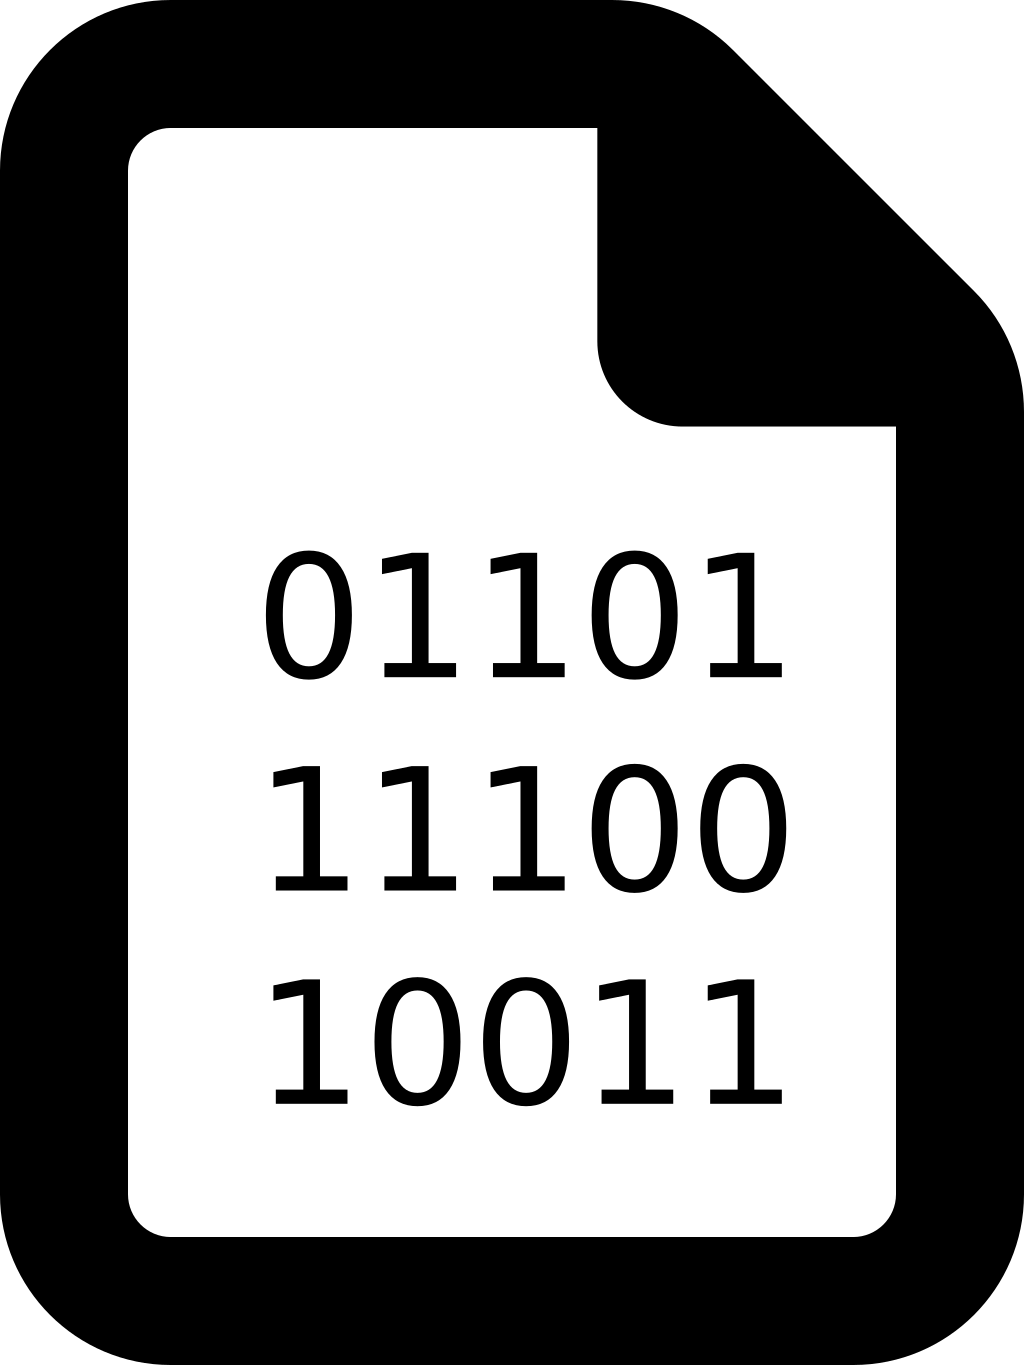
\includegraphics[width=1cm]{pictures/file-bin.png}&
        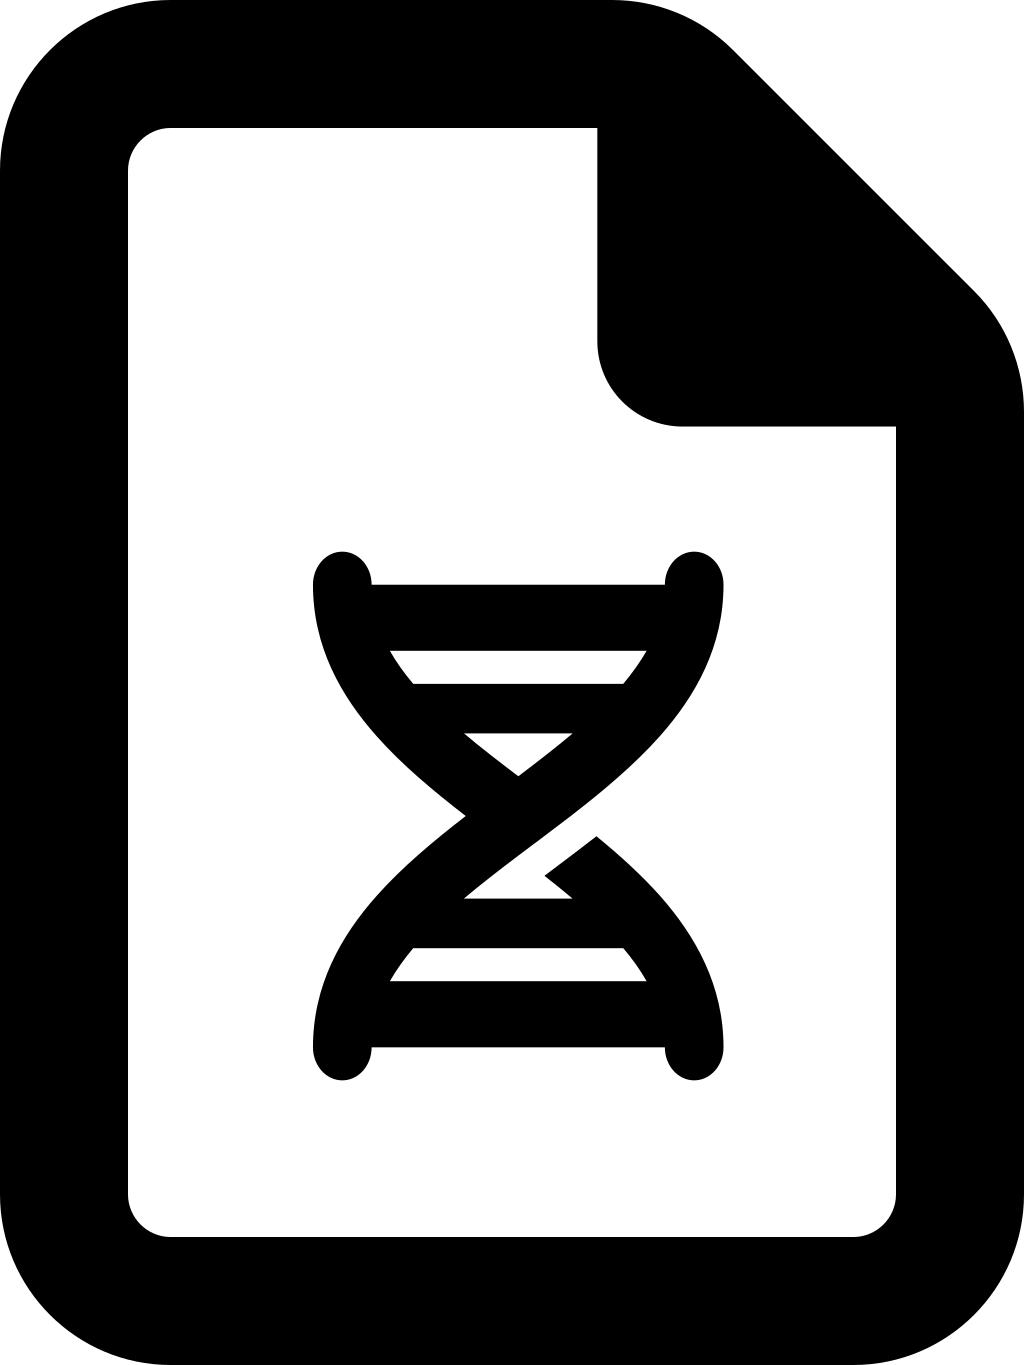
\includegraphics[width=1cm]{pictures/file-dna.png}&
        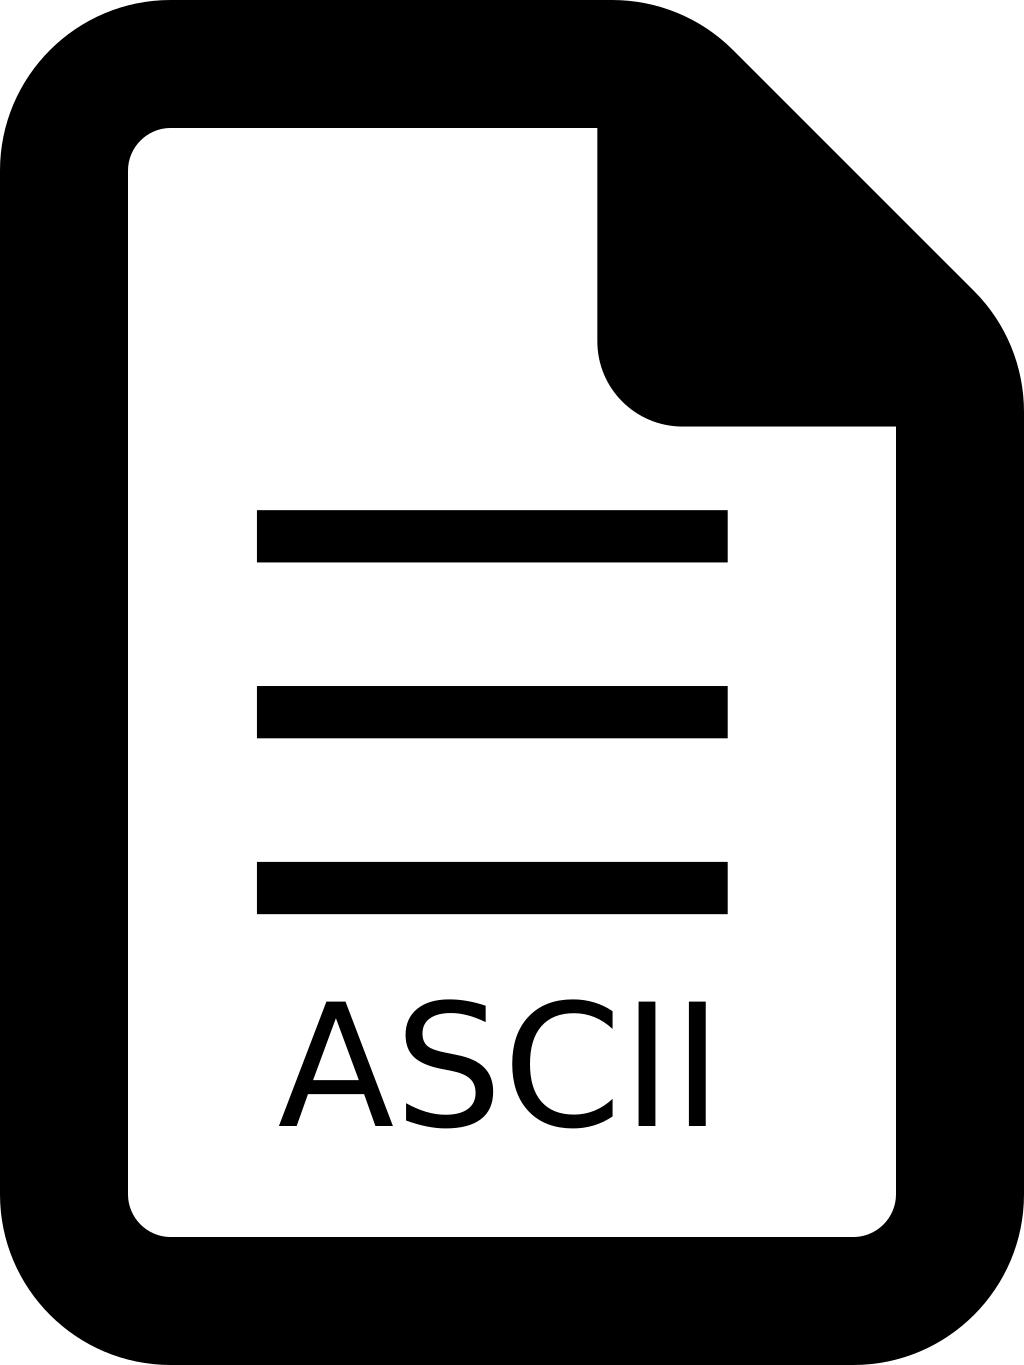
\includegraphics[width=1cm]{pictures/file-ascii.png}&
        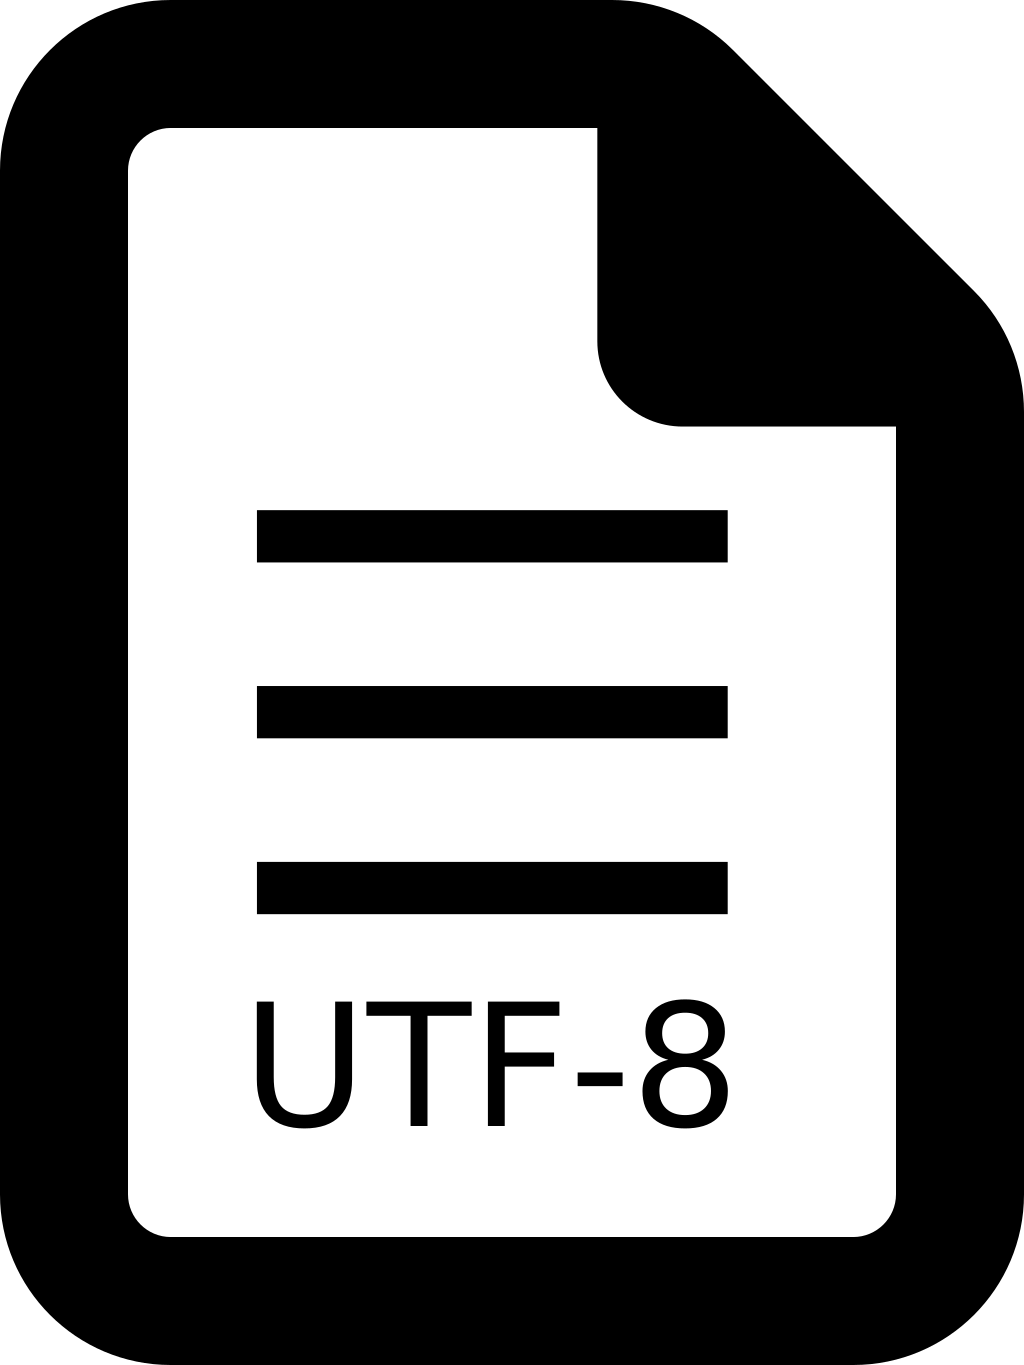
\includegraphics[width=1cm]{pictures/file-utf-8.png}
        \\
        \rule{0pt}{4ex}  
        \emph{Alphabets} & $\Sigma=\{0,1\}$ & $\Sigma=\{\texttt{A,T,C, G}\}$ & $\sigma=128$ & $\sigma = 1,112,064$\\
    \end{tabular}
    \medskip

    Most natural task: Given a pattern $P =$ \texttt{th}, does it occur in  $T$ and where ?

    \begin{center}
        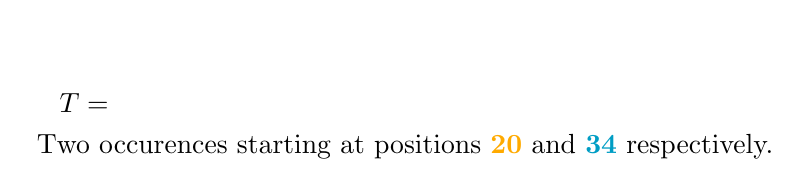
\begin{tikzpicture}[x = 2em]
            \node (t) at (-0.8,0) {\smash{$T=$}$\vphantom{m}$};
            \numberedstring{\stringstruggled};
            \numberedsubstring[myorange]{\stringstruggled}{20}{21};
            \numberedsubstring[myblue]{\stringstruggled}{34}{35};
            \only<1>{
                \node at (20*0.25,-0.5) {
                    Two occurences starting at positions \borange{20} and \bblue{34} respectively.
                };
            }
        \end{tikzpicture}
        \\
    \end{center}

\end{frame}


\begin{frame}{Classic Pattern Matching}

\end{frame}

\begin{frame}{Algorithms vs Data-structures}

\end{frame}

\begin{frame}{Classic Indexing the suffix tree}

\end{frame}

\begin{frame}[noframenumbering,plain]
    \vfill
    \mytitle{Introduction}
    \bigskip
    \begin{center}
        \textbf{\textcolor{gray}{Sketch-based approaches to \borange{process} \bred{massive} string data}}
    \end{center}
    \vfill
\end{frame}

\begin{frame}{Challenges: Processing tasks}
3 categories of task (for this thesis)
Complex Matching
Repetition detection
Similarity Measures and distances
\end{frame}

 \begin{frame}{Complex Matching}
    
 \end{frame}

 \begin{frame}{Repetition detection}
    
 \end{frame}

 \begin{frame}{Similarity Measures and distances}
    
 \end{frame}

\begin{frame}{Challenges: the scale}
    A visualization as done for the loreal poster (starting a the base of wikipedia, which seems already very large)
    And still growing
\end{frame}

\begin{frame}{Challenges: the scale}
    The largerst archive are only searchable by metadata (and already it requires significant efforts...)
    And the 
\end{frame}

\begin{frame}[noframenumbering,plain]
    \vfill
    \mytitle{Introduction}
    \bigskip
    \begin{center}
        \textbf{\textcolor{gray}{\bgreen{Sketch-based} approaches to process massive string data}}
    \end{center}
    \vfill
\end{frame}

\begin{frame}{What is a sketch ?}
    \begin{columns}
        \column{.6\textwidth}
        A \textbf{sketch} is a \bblue{lossless} or \borange{lossy} compression that \textbf{keeps only the essential characteristic of the input} needed to answer a specified type of query.\\
        \column{.35\textwidth}
        
\includegraphics[width=1.8cm]{pictures/photo_betisou.jpg}
        \hspace{0.5cm}
        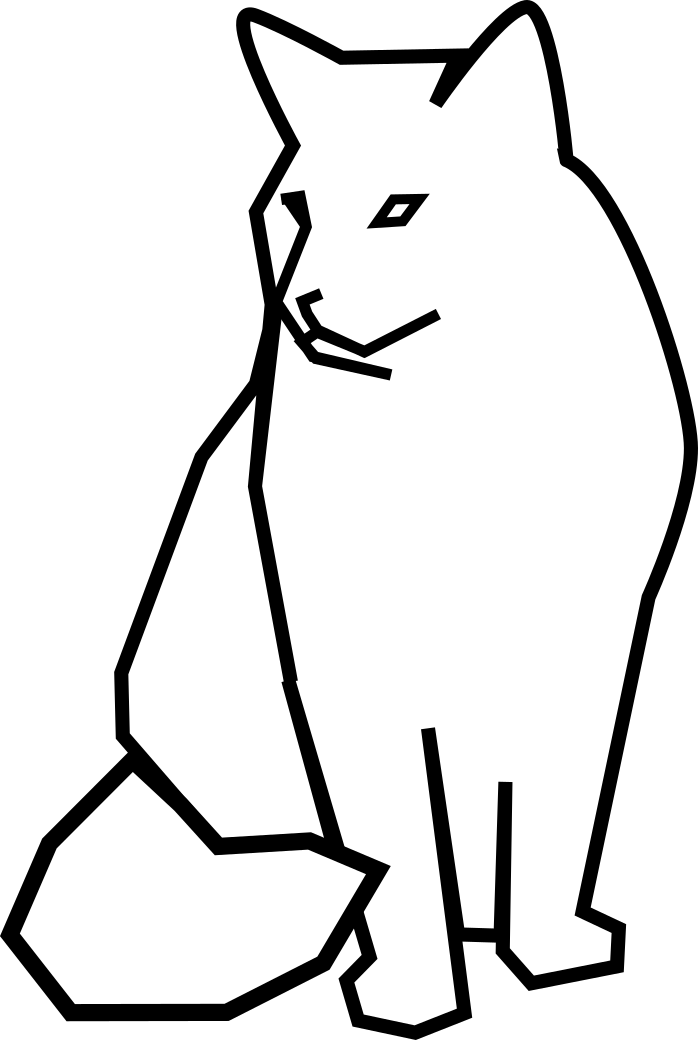
\includegraphics[width=1.8cm]{pictures/betisou.png}\\
        \begin{center}
            "Is this a cat ?"
        \end{center}
    \end{columns}
    \pause

    {\Large Examples:}
    \medskip
    \begin{columns}
        \column{.01\textwidth}
        \column{.48\textwidth}
        {\borange{Lossy: Karp--Rabin fingerprints}}
        \column{.48\textwidth}
        {\bblue{Lossless: Lempel--Ziv factorization}}
    \end{columns}
    
\end{frame}

\begin{frame}{Example of lossy sketch: Karp--Rabin fingerprints}
    \begin{framed}
        Definition: $$ \varphi(P) = P[1]r^{m-1}+P[2]r^{m-2} + \dots + P[m-1]r + P[m] \mod p$$ 
        for $p$ a prime and $r < p$. \pause
        
        Testing if $\varphi(T[i+1..i+m])=\varphi(P)$ can be tested in $\Oh(1)$ and if so the strings match w.h.p.
        \begin{tabular}{l c}
        \textcolor{black}{Sliding window:} & \hspace{1cm}
\includegraphics[width=0.5\textwidth]{pictures/slidding_window.png}
        \end{tabular}
        $$ \varphi(T[i+1..i+m]) = \varphi(T[i..i+m-1])\times r - S[i]r^k + S[i+m] \mod p$$\vspace{-0.5cm}
    \end{framed}
\end{frame}

\begin{frame}{Example of lossless sketch: Lempel--Ziv factorization}
\end{frame}

\begin{frame}{What is a sketch ?}
    \begin{columns}
        \column{.6\textwidth}
        A \textbf{sketch} is a \bblue{lossless} or \borange{lossy} compression that \textbf{keeps only the essential characteristic of the input} needed to answer a specified type of query.\\
        \column{.35\textwidth}
        
\includegraphics[width=1.8cm]{pictures/photo_betisou.jpg}
        \hspace{0.5cm}
        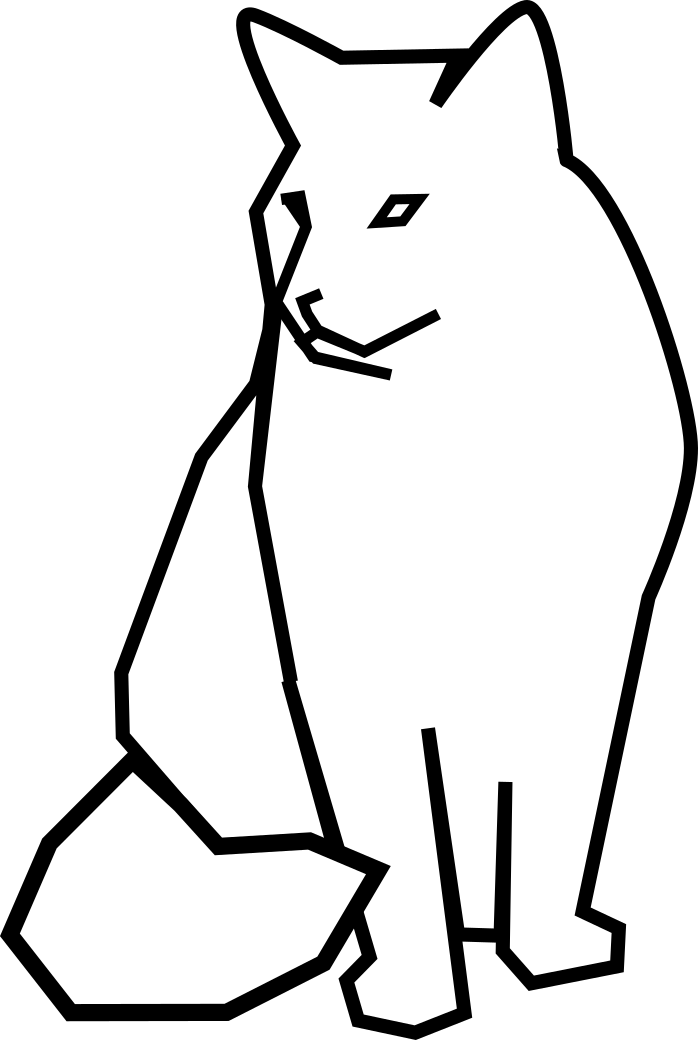
\includegraphics[width=1.8cm]{pictures/betisou.png}\\
        \begin{center}
            "Is this a cat ?"
        \end{center}
    \end{columns}

    {\Large Examples:}
    \medskip
    \begin{columns}
        \column{.01\textwidth}
        \column{.48\textwidth}
        {\borange{Lossy: Karp--Rabin fingerprints}}
        \begin{itemize}
            \item They occupy constant space,  
            \item can check whether two strings match with high probability,
            \item but cannot be used to reconstruct the original string. 
        \end{itemize}
        \column{.48\textwidth}
        {\bblue{Lossless: Lempel--Ziv factorization}}
        \begin{itemize}
            \item It is a very efficient compression in practice (used in \texttt{.png} or \texttt{.zip}),
            \item can reconstruct the original string,
            \item but in the worst case it does not compress. 
        \end{itemize}
    \end{columns}
    
\end{frame}

\begin{frame}{Why should I use sketches and how ?}
    \begin{columns}
        \column{.52\textwidth}
        \small{A \textbf{sketch} is a \bblue{lossless} or \borange{lossy} compression that \textbf{keeps only the essential characteristic of the input} needed to answer a specified type of query.}
        \column{0.05\textwidth}
        \LARGE{$\rightarrow$}
        \column{0.33\textwidth}
            \small{
            Sketches are typically much \bgreen{smaller}, thus can allow \bgreen{scaling to larger} datasets.}
    \end{columns}
    \bigskip
    \pause


    \hspace{-0.5cm} {\large \textcolor{black!30!blue}{Three main approaches in this thesis:}}
    \begin{columns}
        \column{0.33\textwidth}
        \begin{framed}
            \begin{center}
                \textbf{Sketch as input}
            \end{center}
            Operating directly on the sketch given as input (not decompressing).
        \end{framed}
        \column{0.66\textwidth}
        \begin{framed}
            \begin{center}
                \textbf{Sketch as you go}
            \end{center}
            Compute the sketch of the input on the fly and use it later on in your algorithm. 
            \begin{itemize}
                \item For Streaming
                \item For approximation
            \end{itemize}
        \end{framed}
    \end{columns}
\end{frame}


\begin{frame}[noframenumbering,plain]
    \mytitle{Contributions}
    \bigskip
    \begin{columns}
	   \column{.57\textwidth}
      \begin{enumerate}
        \item Streaming Regular Expressions
        \item Gapped Consecutive Matching
        \begin{enumerate}
            \item Compressed Index
            \item Compressed Pattern Matching
        \end{enumerate}
        \item Run-reporting for unordered alphabets
        \item Approximate Longest Common Substring with approximately     mismatches
        \item Pattern Matching for the Dynamic Time Warping distance
        \item Compressing and Indexing Aligned Readsets
      \end{enumerate}
	   \column{.3\textwidth}
        \begin{framed}
            For each:
            \begin{itemize}
                \item Context
                \item Problem
                \item Results
                \item Use of sketches
            \end{itemize}
        \end{framed}
    \end{columns}
\end{frame}

\begin{frame}{Streaming Regular Expressions: Membership and Pattern Matching}
    \begin{columns}
        \column{.6\textwidth}
        \begin{block}{Regular expressions}
            either a character from $\Sigma$ or recursively defined from other regular expressions $R_1$ and $R_2$:
            \pause
            \begin{enumerate}
                \item $R_1 \cdot R_2$ (concatenation),
                \pause
                \item $R_1 | R_2$ (union),
                \pause
                \item $R_1^\ast$ (Kleene star).
            \end{enumerate}
            \pause
        \end{block}
        \column{.3\textwidth}
        Example:
        \begin{center}
            $b(b|ab)^astab$ matches:\\
            \checkmark $bbbbbabab$ \\
            \checkmark $bbbabbbbab$\\
            But does not match $baba$ or $abab$.
        \end{center}
    \end{columns}    
    \pause
    \bigskip
    {
        \beamermathcolor{myblue}
        Given a regexp $R$ and a text $T$, two problems:\\
        \bblue{Membership:} check if $R$ matches $T$.\\
        \bblue{Pattern matching:} check if $R$ matches \textbf{some substring} of $T$.
    }
    \bigskip


    TODO: The classical approach with thomson automatas. 
\end{frame}

\begin{frame}{Streaming Regular Expression: Streaming Model}
\begin{center}
    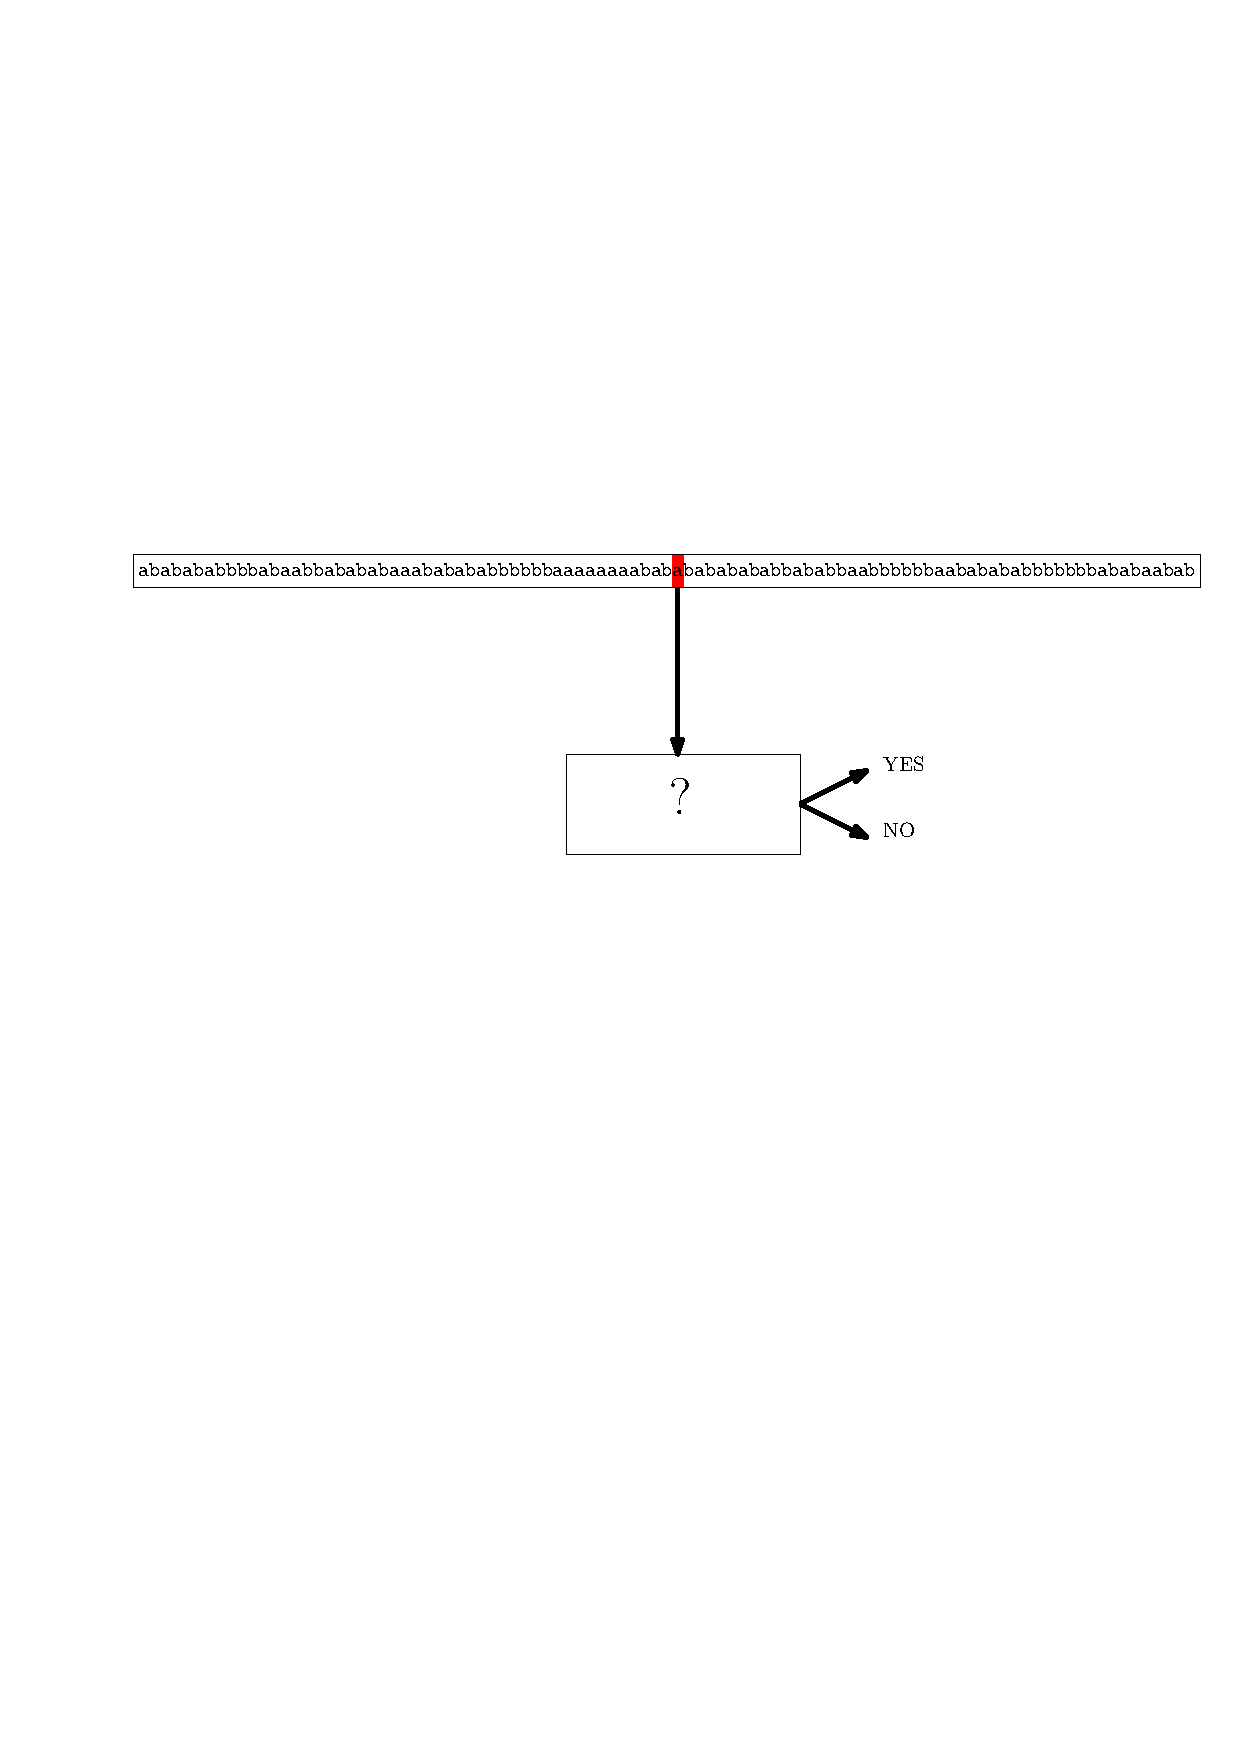
\includegraphics[width=0.7\textwidth]{pictures/stream3}
\end{center}

\medskip

The algorithm first receives and preprocesses the pattern. Next,
it keeps reading characters from a very very long text.

\smallskip
\pause
\begin{enumerate}
\item No delay: After having seen the $i$-th character, immediately report whether there is an
occurrence ending there.
\pause
\item No going back: Not possible to read any of the earlier characters.
\pause
\item Every space counts: No access to the original pattern (unless it has been stored in working space).
\end{enumerate}
\end{frame}

\begin{frame}{Streaming Regular Expression: Our contributions}
    \begin{alertblock}{Dudek, Gawrychowski, Gourdel, Starikovskaya, SODA'22}
        \beamermathcolor{red}
        For any regular expression $R$ with $d$ occurrences of $|$ and $\ast$, we can solve regular expression membership
        and pattern matching using $\Oh(d^{3}\polylog n)$ space and $\Oh(nd^{5}\polylog n)$ time per character.
    \end{alertblock}
\end{frame}

\begin{frame}{A simpler alternative to regular expression: Gapped Consecutive Matching}
    % Regexp are hard to match
    % Many alternative considered 
    % A recent intrest in Gapped Consecutive matching
\end{frame}

\end{document}
